\documentclass{beamer}

\usepackage[english]{babel}
\usepackage{xcolor}
\usepackage{xmpmulti}
\usepackage{amsmath}
\usepackage{dsfont}
\usepackage{multicol}
\usepackage{tikz}
\usepackage{eucal}
\usetikzlibrary{positioning,angles,quotes}
\usepackage{url}
\usepackage{graphicx}
\usepackage{cmbright}
\usepackage{framed}
\usepackage{amssymb}
\usepackage{pifont}

\usetikzlibrary{pgfplots.groupplots,arrows.meta,shadows,positioning,angles,quotes}
\usetikzlibrary{matrix,chains,positioning,decorations.pathreplacing,arrows}
\usepackage{tikz}
\usetikzlibrary{shapes.geometric}
\usetikzlibrary{positioning}
\usepackage{pgfplots}

%\input{epgfplotslibrary{groupplots}
\usetikzlibrary{pgfplots.groupplots,arrows.meta,shadows,positioning,angles,quotes}
\usetikzlibrary{matrix,chains,positioning,decorations.pathreplacing,arrows}

\newcommand{\xmark}{\ding{55}}

\DeclareMathOperator*{\argmax}{arg\,max}
\def\checkmark{\tikz\fill[scale=0.4](0,.35) -- (.25,0) -- (1,.7) -- (.25,.15) -- cycle;} 

\definecolor{Maroon}{cmyk}{0, 0.87, 0.68, 0.32}
\definecolor{RoyalBlue}{cmyk}{1, 0.50, 0, 0}
\definecolor{skymagenta}{rgb}{0.81, 0.44, 0.69}

\newenvironment{takeaway}[1]{%
	\definecolor{shadecolor}{gray}{0.9}%
		\begin{shaded}{\color{skymagenta}\noindent\textsc{#1}}\\%
		}{%
		\end{shaded}%
}



%%%%%% THE FOLLOWING FILE CONTAINS THE STYLE DEFINITIONS %%%%%%
\usepackage[utf8]{inputenc}
\usepackage[export]{adjustbox}

\definecolor{gris}{rgb}{0.92,0.92,0.92}
\definecolor{blau-upc}{rgb}{.192,.365,.506}

\setbeamercolor{titlelike}{fg=blau-upc}
% \setbeamercolor{barra}{bg=white,fg=white}
\setbeamercolor{capcalera}{bg=blau-upc,fg=white}
\setbeamercolor{section in toc}{fg=blau-upc}
\setbeamertemplate{sections/subsections in toc}[circle]
\setbeamertemplate{itemize items}[circle]
\setbeamercolor{item}{fg=blau-upc}
\setbeamertemplate{blocks}[rounded][shadow=true]
\setbeamercolor*{block body}{bg=gris}
\setbeamerfont{block body}{size=\footnotesize}
\setbeamercolor*{block title}{parent=structure,bg=blau-upc,fg=white}

\setbeamersize{text margin left=12mm,text margin right=12mm}
\setbeamertemplate{navigation symbols}{}

\setbeamertemplate{footline}[frame number]{}


\defbeamertemplate*{headline}{infolines theme}
{
	\begin{beamercolorbox}[wd=\paperwidth,ht=6.5mm,right]{white}%
		%
\includegraphics[width = 45mm, height=10mm]{./logotips/visapp}\hspace*{2mm}\vskip0.2ex
	\end{beamercolorbox}
 	\begin{beamercolorbox}[wd=\paperwidth,ht=0.5mm,left]{barra}%
 		\hspace*{1mm}
 	\end{beamercolorbox}
}

\setbeamertemplate{footline}
{
	\hbox{
	\begin{beamercolorbox}[wd=0.1\paperwidth,ht=10mm,left]{}
% 		\hspace*{1ex}
\includegraphics[height=8mm]{./logotips/imperiallogo.pdf}\vskip 2ex
	\end{beamercolorbox}
	\begin{beamercolorbox}[wd=0.8\paperwidth,ht=3ex,center]{}
		\hspace*{4ex}\insertsection\vskip 4ex
	\end{beamercolorbox}
	\begin{beamercolorbox}[wd=0.1\paperwidth,ht=3ex,right]{}
		\insertpagenumber\hspace*{6ex}\vskip 4ex
	\end{beamercolorbox}
	}
}

\setbeamertemplate{title page}
{
	\vbox{}
	\vfill
	\begin{centering}
		{\usebeamerfont{title}\usebeamercolor[fg]{title}\inserttitle}
		\vskip0.2em
		{\usebeamerfont{subtitle}\usebeamercolor[fg]{subtitle}\insertsubtitle}
		\vskip2em\par
		\small\insertauthor\par
		\vskip2em\par
		\tiny\insertdate\vskip1em\par
	\end{centering}
% 	\vfill
}

%\usebackgroundtemplate{\put(-50,-340){\includegraphics[width=10cm]{}}} 

%%%%%%

%%%%%% TITLE, AUTHOR, DATE DEFINITIONS %%%%%%
\title{Model-Free Reinforcement Learning}
\subtitle{Learning Optimal Value Functions}
\author{Matthia Sabatelli}


\date{\today}
%%%%%%

\setbeamertemplate{footline}[frame number]{}

\begin{document}

\frame{\titlepage} 

\frame{\frametitle{Today's Agenda}\tableofcontents}


\begin{frame}{Recap}

	Last lecture we have seen the \textcolor{RoyalBlue}{Dynamic Programming} family of algorithms:
	
	\begin{block}{Key Concepts}
		\begin{itemize}
			\item We have seen what it means to \textcolor{RoyalBlue}{evaluate} a policy $\pi$
			\item Why this task is necessary to be able to \textcolor{RoyalBlue}{improve} $\pi$
			\item How to learn value functions \textcolor{RoyalBlue}{iteratively}
			\item The \textcolor{RoyalBlue}{important role} of the Bellman optimality equations
		\end{itemize}
		
	\end{block}

\end{frame}

\begin{frame}{Model-Free Reinforcement Learning}
	\section{Model-Free Reinforcement Learning}
	We have therefore derived:

	\begin{itemize}
		\item How to \textcolor{RoyalBlue}{estimate} an optimal value function and \textcolor{RoyalBlue}{discover} an optimal policy $\pi^*$ 
		\item We did this under the assumption that the environment $\mathcal{M}=\langle \mathcal{S},\mathcal{A},\mathcal{P},r\rangle$ was \textcolor{RoyalBlue}{known}
	\end{itemize}

			\begin{block}{Plot Twist!}
				We will now consider situations where \textcolor{Maroon}{no complete knowledge} is available:
				\begin{itemize}
					\item Set of possible states $\mathcal{S}$ \textcolor{green}{\checkmark} 
					\item Set of possible actions $\mathcal{A}$ \textcolor{green}{\checkmark}
					\item Transition Function $\mathcal{P}:\mathcal{S}\times\mathcal{A}\times\mathcal{S}\rightarrow[0,1]$ \textcolor{red}{\xmark}
					\item Reward Function $\Re:\mathcal{S}\times\mathcal{A}\times\mathcal{S}\rightarrow \mathbb{R}$ \textcolor{red}{\xmark}
				\end{itemize}
			\end{block}
\end{frame}


\begin{frame}{Model-Free Reinforcement Learning}
	When parts of of the MDP $\mathcal{M}$ are \textcolor{Maroon}{unknown} we do not deal with Dynamic Programming methods anymore but with Reinforcement Learning algorithms!
	\begin{itemize}
		\item We need to overcome the \textcolor{Maroon}{lack of information} of $\mathcal{M}$
		\item We can do this through \textcolor{RoyalBlue}{experience}
		\item Gathering experience means \textcolor{RoyalBlue}{sampling} states $s$, actions $a$ and rewards $r$ from the environment
		\item Recall the concept of \textcolor{RoyalBlue}{trajectory} $\tau$ $\langle s_t,a_t,r_t,s_{t+1} \rangle$ seen in Lecture 1! 
	\end{itemize}
\end{frame}


\begin{frame}{Model-Free Reinforcement Learning}
	What does it mean in practice?
	\begin{itemize}
		\item We do not know \textcolor{Maroon}{the consequences} of our actions
		\item We do not know the \textcolor{Maroon}{dynamics} of the environment we are interacting with
		\item We are no longer \textcolor{Maroon}{computing} value functions but rather \textcolor{RoyalBlue}{learning} them
	\end{itemize}

	\bigskip

	The transition function $\mathcal{P}$ and the reward function $\Re$ are usually called the \textcolor{RoyalBlue}{model} of the environment
	
	\bigskip
	
	$\mathcal{P}$ and $\Re$ can be \textcolor{RoyalBlue}{learned} $\Rightarrow$ model-based Reinforcement Learning

\end{frame}


\begin{frame}{Model-Free Reinforcement Learning}
	Why is model-free Reinforcement Learning so interesting?
	\begin{itemize}
		\item We learn without any \textcolor{RoyalBlue}{prior knowledge} of the environment
		\item Trajectories, and therefore \textcolor{RoyalBlue}{experience}, is sufficient for learning
		\item We "only" need a value function $Q(s,a)$, which is arguably \textcolor{RoyalBlue}{easier} to learn than the model
	\end{itemize}

	\bigskip

	The effectiveness of model-free Reinforcement Learning algorithms \textcolor{Maroon}{highly depends} from how much experience the agent is able to gather!

\end{frame}


\begin{frame}{Monte Carlo (MC) Methods}
	\section{Monte Carlo Methods}
		Monte Carlo methods:
		\begin{itemize}
			\item Can be used for learning $V^\pi(s)$ as well as $Q^\pi(s,a)$ 
			\item Although in this lecture we only focus on learning $V^\pi(s)$
			\item The key idea is to learn through \textcolor{RoyalBlue}{sampling returns}
		\end{itemize}

	\begin{block}{Assumption!}
		We assume that we are always dealing with \textcolor{RoyalBlue}{episodic tasks} i.e. episodes eventually \textcolor{Maroon}{terminate}.
		\begin{align*}
			\langle(s_t,a_t,r_t,s_{t+1})\rangle, t=0,..., T-1
		\end{align*}
	\end{block}
\end{frame}

\begin{frame}{Monte Carlo (MC) Methods}
	Let us consider the notion of expected discounted return introduced in Lecture 1:
	\begin{align*}
		G_t & = r_t+\gamma r_{t+1}, \gamma^{2} r_{t+2} + ... \\
			& = \sum_{k=0}^{\infty}\gamma^{k} r_{t+k+1}.	
	\end{align*}

	\begin{itemize}
		\item The \textcolor{Maroon}{goal} is to learn the state-value function of a given policy $V^\pi(s)$: \textcolor{RoyalBlue}{Monte Carlo Prediction} 
		\item We do this with respect to the $G_t$ that is obtained by following $\pi$
	\end{itemize}
\end{frame}


\begin{frame}{Monte Carlo (MC) Methods}
	Learning $V^{\pi}(s)$ involves the following \textcolor{RoyalBlue}{steps}:
	\begin{itemize}
		\item Before learning, each state has its own value $V(s_t)$
		\item We follow policy $\pi$ until an episode terminates 
		\item We compute the discounted return $G_t$ that was obtained by $\pi$
	\end{itemize}

	\begin{block}{Monte Carlo (MC) Update Rule}
		We change the value of each state $V(s_t)$ based on $G_t$
		\begin{align*}
			V(s_t) := V(s_t) + \alpha \:[G_t-V(s_t)].
		\end{align*}
		where $\alpha \in [0,1]$ is the learning rate parameter.
	\end{block}

\end{frame}


\begin{frame}{Monte Carlo (MC) Methods}
	Let us consider the following MDP:

	\centering
	\tikzset{
    ->, 
    level distance = 22em,
    minimum size=2em,
    %edge from parent/.style={draw,thick},
    level 1/.style={sibling distance=6em},
    level 2/.style={sibling distance=3em},
    thick/.style = {line width=1.5pt},
    extra thick/.style = {line width=3.5pt},
    red node/.style={shape=circle,draw=red,fill=red!40,thick,inner sep=1.2},
    blue node/.style={shape=circle,draw=blue,fill=blue!40,thick,inner sep=1.2}
}

\tikzstyle{round}=[thick,draw=black,circle]

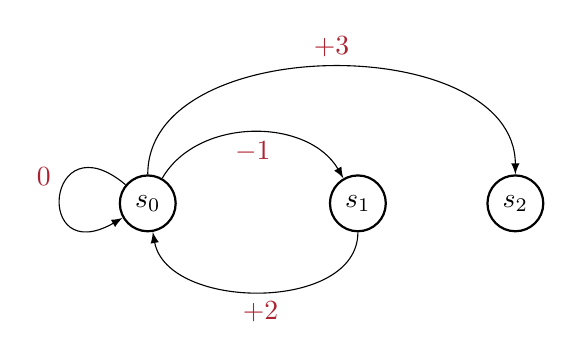
\begin{tikzpicture}[auto,node distance=58mm,>=latex]
    \tikzstyle{round}=[thick,draw=black,circle]
    \node[round] (s0) {$s_0$};
    \node[round, above=10mm, right=23mm] (s1) {$s_1$};
    \node[round, below=30mm, right=43mm] (s2) {$s_2$};

    \draw[->] (s0) [out=60,in=120] to node {} node [swap] {\textcolor{Maroon}{$-1$}} (s1);
    \draw[->] (s1) [out=-90,in=-80] to node {\textcolor{Maroon}{$+2$}} node [swap] {} (s0);
    \draw[->] (s0) [out=90,in=90] to node {\textcolor{Maroon}{$+3$}} node [swap] {} (s2);
    \draw[->] (s0) [out=140,in=210,loop] to node {} node [swap] {\textcolor{Maroon}{$0$}} (s0);




\end{tikzpicture}


	\begin{itemize}
		\item We have policy $\pi: s0\rightarrow s1 \rightarrow s0 \rightarrow s2$
		\item $\pi$ results in the sequence of rewards $-1, +2, +3$
		\item The starting value of each state is $0$, $\gamma=0.99$ and $\alpha=0.5$
	\end{itemize}
	
\end{frame}


\begin{frame}{Monte Carlo (MC) Methods}
	
	We know that $G_t$ for starting in $s0$ is 
	\begin{align*}
		G_t & = \sum_{k=0}^{\infty}\gamma^{k} r_{t+k+1} \\ 
		    & = -1+\gamma2+\gamma^{2}3 \approx 3.92
	\end{align*}

	Therefore
	\begin{align*}
		V(s_t) & := V(s_t) + \alpha \:[G_t-V(s_t)] \\
		V(0) & := V(0) + \alpha \:[3.92-V(0)] \approx 1.96
	\end{align*}

\end{frame}

\begin{frame}{Monte Carlo (MC) Methods}
	More about Monte Carlo Methods:
	\begin{itemize}
		\item We have only considered the \textcolor{RoyalBlue}{prediction} case of learning $V^\pi(s)$
		\item Monte Carlo \textcolor{RoyalBlue}{control} algorithms learn an approximation of $\pi^*$ through $Q^{\pi}(s,a)$
		\item They follow the ideas of \textcolor{RoyalBlue}{Dynamic Programming} seen in the previous lecture 
		\item The key idea of \textcolor{Maroon}{sampling real returns} remains!
	\end{itemize}

\end{frame}

\begin{frame}{Monte Carlo (MC) Methods}
	Pros \& Cons of Monte Carlo Methods:
	\begin{itemize}
		\item Yield \textcolor{RoyalBlue}{unbiased} updates thanks to $G_t$ \textcolor{green}{\checkmark}
		\item \textcolor{RoyalBlue}{Scale well} to function approximators \textcolor{green}{\checkmark}
		\item Learning can be very \textcolor{Maroon}{slow} as one has to wait until the very end of an episode \textcolor{red}{\xmark}
		\item There can be \textcolor{Maroon}{large variance} in the value updates \textcolor{red}{\xmark}
	\end{itemize}
\end{frame}


\begin{frame}{Temporal Difference (TD) Learning}
	\section{Temporal Difference Learning}
	\begin{center}
		\textit{"The simplest and most elegant idea of Reinforcement Learning ..."}
	\end{center}
\end{frame}


\begin{frame}{Temporal Difference (TD) Learning}
	With TD-Learning methods we \textcolor{Maroon}{do not} have to wait until the end of an episode before updating a value estimate
	\begin{itemize}
		\item We only need to wait until the \textcolor{RoyalBlue}{next step}
		\item At $t+1$ we immediately create a \textcolor{RoyalBlue}{target} for learning called the TD-target
		\item We do this by using the observed reward \textcolor{RoyalBlue}{$r_t$} and a future value estimate e.g. \textcolor{RoyalBlue}{$V(s_{t+1})$}
	\end{itemize}	
\end{frame}

\begin{frame}{Temporal Difference (TD) Learning}
	Let us again consider the problem of estimating $V^{\pi}(s)$:
	\begin{block}{TD Prediction}
		We change the value of each state $V(s_t)$ with respect to $t+1$ only:
		\begin{align*}
			V(s_t):= V(s_t) + \alpha \big[r_t + \gamma V(s_{t+1}) - V(s_t)\big].
		\end{align*}
	\end{block}
	
	\begin{itemize}
		\item It is clear that we only learn by \textit{looking ahead} in the future one single step
		\item This is called $\text{TD}(0)$ or \textit{one-step TD}
	\end{itemize}

\end{frame}


\begin{frame}{Temporal Difference (TD) Learning}
	The key idea of TD-Learning it to learn through \textcolor{RoyalBlue}{bootsrapping}:
	\begin{itemize}
		\item We update the value of a state with respect to the value of its \textcolor{RoyalBlue}{successor} state only
		\item Ideally we would like to use $V^{\pi}(s_{t+1})$ for learning but it is unfortunately \textcolor{Maroon}{unknown}
	\end{itemize}	
	\begin{align*}
		V(s_t):= V(s_t) + \alpha \big[r_t + \gamma V^{\pi}(s_{t+1}) - V(s_t)\big].
	\end{align*}
	Therefore we \textcolor{RoyalBlue}{replace} it with a guess instead:
	\begin{align*}
		V(s_t):= V(s_t) + \alpha \big[r_t + \gamma V(s_{t+1}) - V(s_t)\big].
	\end{align*}
	
\end{frame}


\begin{frame}{Temporal Difference (TD) Learning}
	The key idea of TD-Learning it to learn through \textcolor{RoyalBlue}{bootsrapping}:
	\begin{itemize}
		\item We update the value of a state with respect to the value of its \textcolor{RoyalBlue}{successor} state only
		\item Ideally we would like to use $V^{\pi}(s_{t+1})$ for learning but it is unfortunately \textcolor{Maroon}{unknown}
	\end{itemize}
	\begin{align*}
		V(s_t):= V(s_t) + \alpha \big[r_t + \gamma \textcolor{red}{V^{\pi}(s_{t+1})} - V(s_t)\big].
	\end{align*}
	Therefore we \textcolor{RoyalBlue}{replace} it with a guess instead:
	\begin{align*}
		V(s_t):= V(s_t) + \alpha \big[r_t + \gamma \textcolor{RoyalBlue}{V(s_{t+1})} - V(s_t)\big].
	\end{align*}
	
\end{frame}

\begin{frame}{Temporal Difference (TD) Learning}
	Let us go back to the previous MDP:
	\begin{center}
	\tikzset{
    ->, 
    level distance = 22em,
    minimum size=2em,
    %edge from parent/.style={draw,thick},
    level 1/.style={sibling distance=6em},
    level 2/.style={sibling distance=3em},
    thick/.style = {line width=1.5pt},
    extra thick/.style = {line width=3.5pt},
    red node/.style={shape=circle,draw=red,fill=red!40,thick,inner sep=1.2},
    blue node/.style={shape=circle,draw=blue,fill=blue!40,thick,inner sep=1.2}
}

\tikzstyle{round}=[thick,draw=black,circle]

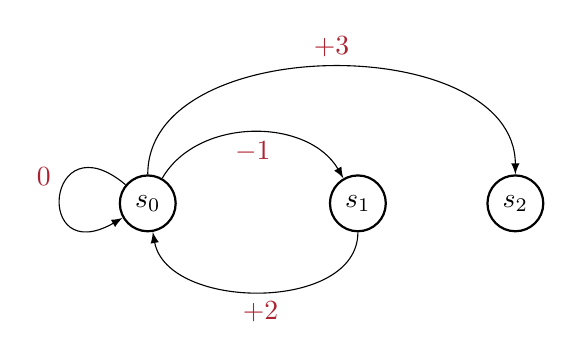
\begin{tikzpicture}[auto,node distance=58mm,>=latex]
    \tikzstyle{round}=[thick,draw=black,circle]
    \node[round] (s0) {$s_0$};
    \node[round, above=10mm, right=23mm] (s1) {$s_1$};
    \node[round, below=30mm, right=43mm] (s2) {$s_2$};

    \draw[->] (s0) [out=60,in=120] to node {} node [swap] {\textcolor{Maroon}{$-1$}} (s1);
    \draw[->] (s1) [out=-90,in=-80] to node {\textcolor{Maroon}{$+2$}} node [swap] {} (s0);
    \draw[->] (s0) [out=90,in=90] to node {\textcolor{Maroon}{$+3$}} node [swap] {} (s2);
    \draw[->] (s0) [out=140,in=210,loop] to node {} node [swap] {\textcolor{Maroon}{$0$}} (s0);




\end{tikzpicture}

	\end{center}

	\begin{itemize}
		\item We again have policy $\pi: s0\rightarrow s1 \rightarrow s0 \rightarrow s2$
		\item $\pi$ results in the sequence of rewards $-1, +2, +3$
		\item The starting value of each state is $0$, $\gamma=0.99$ and $\alpha=0.5$
	\end{itemize}
	
\end{frame}


\begin{frame}{Temporal Difference (TD) Learning}
	\begin{center}
	\tikzset{
    ->, 
    level distance = 22em,
    minimum size=2em,
    %edge from parent/.style={draw,thick},
    level 1/.style={sibling distance=6em},
    level 2/.style={sibling distance=3em},
    thick/.style = {line width=1.5pt},
    extra thick/.style = {line width=3.5pt},
    red node/.style={shape=circle,draw=red,fill=red!40,thick,inner sep=1.2},
    blue node/.style={shape=circle,draw=blue,fill=blue!40,thick,inner sep=1.2}
}

\tikzstyle{round}=[thick,draw=black,circle]

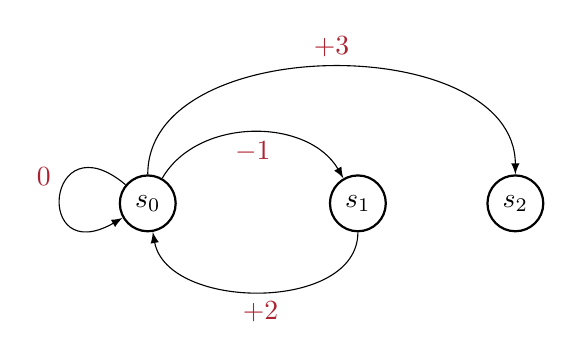
\begin{tikzpicture}[auto,node distance=58mm,>=latex]
    \tikzstyle{round}=[thick,draw=black,circle]
    \node[round] (s0) {$s_0$};
    \node[round, above=10mm, right=23mm] (s1) {$s_1$};
    \node[round, below=30mm, right=43mm] (s2) {$s_2$};

    \draw[->] (s0) [out=60,in=120] to node {} node [swap] {\textcolor{Maroon}{$-1$}} (s1);
    \draw[->] (s1) [out=-90,in=-80] to node {\textcolor{Maroon}{$+2$}} node [swap] {} (s0);
    \draw[->] (s0) [out=90,in=90] to node {\textcolor{Maroon}{$+3$}} node [swap] {} (s2);
    \draw[->] (s0) [out=140,in=210,loop] to node {} node [swap] {\textcolor{Maroon}{$0$}} (s0);




\end{tikzpicture}

	\end{center}

	Our first state transition is $s0 \rightarrow s1$

	\begin{align*}
		V(s_t) & := V(s_t) + \alpha \big[r_t + \gamma V(s_{t+1}) - V(s_t)\big] \\
		V(s0) & := V(s0) + \alpha \big[r_t + \gamma V(s1) - V(s0)\big] \\ 
		V(s0) & := -0.5
	\end{align*}

\end{frame}

\begin{frame}{Temporal Difference (TD) Learning}
	What is so cool about the TD Learning update rule?

	\begin{align*}
		V(s_t) & := V(s_t) + \alpha \big[r_t + \gamma V(s_{t+1}) - V(s_t)\big] \\
	\end{align*}

	\begin{center}
	\textcolor{RoyalBlue}{\textit{We are learning by guessing!}}
	\end{center}

	\bigskip

	\begin{itemize}
		\item We want to learn $V(s_t)$ with respect to $V(s_{t+1})$
		\item But $V(s_{t+1})$ is as unknown as $V(s_t)$
		\item We use the information provided by the environment $r_t$ immediately to construct the \textcolor{RoyalBlue}{TD-error} $\delta_t$
	\end{itemize}

	\begin{align*}
		V(s_t) & := V(s_t) + \alpha \big[\underbrace{r_t + \gamma V(s_{t+1})-V(s_t)}_{\textcolor{blue}{\delta_t}}\big] \\
	\end{align*}
\end{frame}

\begin{frame}{Temporal Difference (TD) Learning}
	Why are the TD-errors \textcolor{blue}{$\delta_t$} so important?
	\begin{itemize}
		\item They allow us to start learning \textcolor{RoyalBlue}{immediately} 
		\item They separate RL algorithms into two \textcolor{RoyalBlue}{families} of techniques: \textit{off-policy} and \textit{on-policy} techniques
		\item Each family comes with its own \textcolor{RoyalBlue}{convergence properties}
	\end{itemize}

	\bigskip

	To know more about these families let us consider the problem of learning the state-action value function $Q^{\pi}(s,a)$
	
	\begin{align*}
     	Q^{\pi}(s,a)=\mathds{E}\bigg[\sum_{k=0}^{\infty}\gamma^{k}r_{t+k} \bigg| s_t = s, a_t=a, \pi\bigg].
	\end{align*}
\end{frame}

\begin{frame}{Temporal Difference (TD) Learning}
	The arguably most popular algorithm for learning $Q^{\pi}(s,a)$ is \textcolor{RoyalBlue}{Q-Learning} (Watkins \& Dayan, 1992)

	\begin{itemize}
		\item Is an \textit{off-policy} learning algorithm 
		\item Able of converging to the optimal state-action value function $Q^{*}(s,a)$ with probability $1$
		\item Works by keeping track of an estimate of the state-action value function $Q: \mathcal{S} \times \mathcal{A} \rightarrow \Re$
	\end{itemize}

	\begin{block}{Q-Learning}
		The update rule of each visited state-action pair used by Q-Learning is:
		\begin{align*}
			Q(s_t,a_t):=Q(s_t,a_t) + \alpha\Big[r_t + \gamma \:\underset{a\in \mathcal{A}}{\max} Q(s_{t+1},a_t) - Q(s_t, a_t) \Big].
		\end{align*}
	\end{block}

\end{frame}

\begin{frame}{Temporal Difference (TD) Learning}

	How does Q-Learning work?

	\begin{align*}
		Q(s_t,a_t):=Q(s_t,a_t) + \alpha\Big[\underbrace{r_t + \gamma \:\underset{a\in \mathcal{A}}{\max} Q(s_{t+1},a_t) - Q(s_t, a_t)}_{\textcolor{blue}{\delta_t}}\Big]
	\end{align*}

	\begin{itemize}
		\item \onslide<+-> We create the TD-error $\delta_t$ by using the \textcolor{Maroon}{$\underset{a\in \mathcal{A}}{\max}$} operator 
		\item \onslide<+-> We \textcolor{Maroon}{always} update $Q(s_t,a_t)$ with respect to a greedy policy
		\item \onslide<+-> Even if the agent is exploring the environment, learning is done \textcolor{Maroon}{greedily} $\rightarrow$ \textit{off-policy} learning
	\end{itemize}

\end{frame}



\begin{frame}{Temporal Difference (TD) Learning}

	We can also learn the $Q^{\pi}(s,a)$ function in a way which is more similar to how we learned $V^{\pi}(s)$ beforehand: \textcolor{RoyalBlue}{SARSA} (Rummery \& Niranjan, 1994)

	\begin{itemize}
		\item Is an \textit{on-policy} learning algorithm
		\item Also works by keeping track of $Q: \mathcal{S} \times \mathcal{A} \rightarrow \Re$ 
		\item Has different convergence properties 

	\end{itemize}

	\begin{block}{SARSA}
		The update rule of each visited state-action pair used by SARSA is:
		\begin{align*}
			Q(s_t,a_t):=Q(s_t,a_t) + \alpha\Big[r_t + \gamma \:Q(s_{t+1},a_{t+1}) - Q(s_t, a_t) \Big].
		\end{align*}
	\end{block}
\end{frame}

\begin{frame}{Temporal Difference (TD) Learning}

		If we take a look at SARSA's TD-error ...

		\begin{align*}
			Q(s_t,a_t):=\underbrace{Q(s_t,a_t) + \alpha\Big[r_t + \gamma \: Q(s_{t+1},a_{t+1})}_{\textcolor{blue}{\delta_t}} - Q(s_t, a_t) \Big]
		\end{align*}


		\begin{itemize}
			\item \onslide<+-> We \textcolor{Maroon}{do not use} the $\max$ operator anymore
			\item \onslide<+-> We learn with respect to the next state that is visited by the agent $s_{t+1}$, which might or \textcolor{Maroon}{might not} (important!) correspond to a greedy policy
			\item \onslide<+-> As we are always taking into account the actions chosen by the agent $Q(s_{t+1}, a_{t+1})$ we learn $\rightarrow$ \textit{on-policy}
		\end{itemize}

\end{frame}



\begin{frame}{Temporal Difference (TD) Learning}

		If we take a look at SARSA's TD-error ...

		\begin{align*}
			Q(s_t,a_t):=\underbrace{Q(\textcolor{red}{s_t,a_t}) + \alpha\Big[\textcolor{red}{r_t} + \gamma \: Q(\textcolor{red}{s_{t+1},a_{t+1}})}_{\textcolor{blue}{\delta_t}} - Q(s_t, a_t) \Big]
		\end{align*}


		\begin{itemize}
			\item We \textcolor{Maroon}{do not use} the $\max$ operator anymore
			\item We learn with respect to the next state that is visited by the agent $s_{t+1}$, which might or \textcolor{Maroon}{might not} (important!) correspond to a greedy policy
			\item As we are always taking into account the actions chosen by the agent $Q(s_{t+1}, a_{t+1})$ we learn $\rightarrow$ \textit{on-policy}
		\end{itemize}

\end{frame}



\begin{frame}{Temporal Difference (TD) Learning}
	
	\begin{takeaway}{Quiz Time!}
		Imagine an algorithm which learns the state-value function $V^{\pi}(s)$ as follows 
		\begin{align*}
			V(s):= V(s) + \alpha \big[r_{t} + \gamma V(s_{t+1}) - V(s_t) \big]
		\end{align*}
		and the state-action value function $Q^{\pi}(s,a)$ as follows:
		\begin{align*}
			Q(s_{t}, a_{t}):= Q(s_{t}, a_{t}) + \alpha \big[r_{t} + \gamma V(s_{t+1}) - Q(s_{t}, a_{t}) \big].
		\end{align*}
	\end{takeaway}

	\begin{itemize}
		\item What is the TD-target of this algorithm?
		\item Is this an \textit{off-policy} or \textit{on-policy} learning algorithm?
	\end{itemize}

\end{frame}


\begin{frame}{Temporal Difference (TD) Learning}
	
	\begin{takeaway}{Quiz Time!}
		Now imagine an algorithm which learns the state-value function $V^{\pi}(s)$ as follows 
		\begin{align*}
			V(s):= V(s) + \alpha \big[r_{t} + \gamma \: \underset{a\in \mathcal{A}}{\max}Q(s_{t+1},a_t) - V(s_t) \big]
		\end{align*}
		and the state-action value function $Q^{\pi}(s,a)$ as follows:
		\begin{align*}
			Q(s_{t}, a_{t}):= Q(s_{t}, a_{t}) + \alpha \big[r_{t} + \gamma V(s_{t+1}) - Q(s_{t}, a_{t}) \big].
		\end{align*}
	\end{takeaway}


	\begin{itemize}
		\item What is the TD-target of this algorithm?
		\item Is this an \textit{off-policy} or an \textit{on-policy} learning algorithm?
	\end{itemize}


\end{frame}


\begin{frame}{Temporal Difference (TD) Learning}
	Pros \& Cons of TD-Learning methods:
	\begin{itemize}
		\item They \textcolor{Maroon}{do not} yield unbiased estimates \textcolor{red}{\xmark}
		\item But there is \textcolor{RoyalBlue}{small variance} in the updates \textcolor{green}{\checkmark}
		\item Learning starts \textcolor{RoyalBlue}{faster} \textcolor{green}{\checkmark}
		\item It can be \textcolor{Maroon}{complicated} to combine them with non-linear function approximators \textcolor{red}{\xmark}
	\end{itemize}

	Both approaches can be combined resulting in $\text{TD}(\lambda)$ algorithms!

	\bigskip

	$\Rightarrow$ TD-Learning methods empirically work better than MC algorithms but a formal proof about why this is the case is missing ...

\end{frame}

\begin{frame}{Final Slide!}
	\begin{takeaway}{Lecture Takeaway}
		\begin{itemize}
			\item What happens when parts of the Markov Decision Process are unknown
			\item Dynamic Programming $\rightarrow$ Reinforcement Learning
			\item Two families of model-free Reinforcement Learning algorithms
			\item We have seen the difference between \textit{on-policy} and \textit{off-policy} learning
		\end{itemize}

	\end{takeaway}
\end{frame}

%============================================================================
\end{document}
